%!TEX root = ../main.tex

\chapter{ 線形計画モデル}
問題の対象となるモデルを線形な等式・不等式制約の集合として表現できる場合，
線形計画法を適用することが合理的である．線形計画法を用いる主な利点として，
変数を連続値として扱えるため，離散化誤差が生じない点が挙げられる．本章では，まず線形計画法を用いたモデル化について述べる．

\section{本研究での時間の扱い}
計画対象となる期間の先頭の時刻を時刻0とし，当該期間を等間隔に$K$個の区間に分割する．
分割された各々の区間の区間幅を$\Delta t$とし，これ以降この区間のことを以降「期」とよぶ．
特に，時刻$(k-1)\Delta t$から時刻$k\Delta t$までの区間のことを「$k$期」と定義する．

以降，各々の変数について期の情報を伴う場合は，その変数に$1,\dots,K$のインデックスを付す．その下で，
太陽光発電電力量や電力需要量など，期間で定義される変数$E_k(k=1,\dots ,K)$は$k$期における総量として定義し，
蓄電池の残量など，時点の状態で定義される変数$S_k(k=1, \dots , K)$については各々の期の末尾で定義する．
なお，例外的に計画期間における初期状態は$S_0$のように表す．時間の扱いについてのイメージを図\ref{fig:time_dig_lp}に示す．

\begin{figure}[h]
	\centering
 	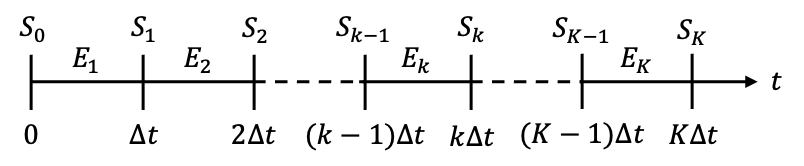
\includegraphics[width=155mm]{../figure/time_dig.png}
 	\caption{Period and measured time}
 	\label{fig:time_dig_lp}
\end{figure}

\section{モデルの要素}
\ref{sec:object}節で示したモデルの要素(\IS を付して記す)と，これらの要素に付随する定数(\IB を付して記す)，変数(\IC を付して表す)を列挙する．
モデル中の定数・変数と電力グリッドとの関係を図\ref{fig:variables_lp}に示す．
赤色の文字は決定変数，青色の文字は従属変数，緑色の文字は外生変数である．
なお，定数・変数の傍らに灰色で付記された文字は，その定数・変数が後述する当該のケースを採用した場合にのみ現れることを表している．

\begin{itemize}
 	\item[\IS] 太陽光発電設備G
		\begin{itemize}
		 	\item[\IB] 太陽光発電電力量(変換前) $g^{\rm P1}_{k}$
  			\item[\IC] 太陽光発電電力量(変換後) $g^{\rm P2}_{k}$
		\end{itemize}	
	 \item[\IS] 電力消費機器D$^{\rm A}$
	 	\begin{itemize}
		 	\item[\IC] 電力需要量A (変換前) $d^{\rm A1}_{k}$
 			\item[\IB] 電力需要量A (変換後) $d^{\rm A2}_{k}$
		\end{itemize}
 	\item[\IS] 電力消費機器D$^{\rm B}$
	 	\begin{itemize}
		 	\item[\IC] 電力需要量B (変換前) $d^{\rm B1}_{k}$
 			\item[\IB] 電力需要量B (変換後) $d^{\rm B2}_{k}$
		\end{itemize}	
 	\item[\IS] 電力消費機器D$^{\rm C}$
	 	\begin{itemize}
		 	\item[\IC] 電力需要量C (変換前) $d^{\rm C1}_{k}$
 			\item[\IB] 電力需要量C (変換後) $d^{\rm C2}_{k}$
		\end{itemize}
 	\item[\IS] 電力消費機器（自己託送先）D$^{\rm D}$
 	\begin{itemize}
   		\item[\IB] 自己託送先が必要とする電力 $d^{\rm D}$
   		\item[\IB] 自己託送先へ託送することのインセンティブ係数 $p^{\rm D}$   
		\item[\IC] 自己託送先への託送量 (変換前) $d^{\rm D1}_{k}$
 		\item[\IC] 自己託送先への託送量(変換後) $d^{\rm D2}_{k}$
  	\end{itemize} 
 	\item[\IS] 蓄電池B$^{\rm F}$
  		\begin{itemize}
   			\item[\IB] 蓄電池の最大容量 $\overline{b}^{\rm F}$
			\item[\IB] 蓄電池の初期残量 $b^{\rm F}_{0}$
		  	\item[\IC] 蓄電池の(期末の)残量 $b^{\rm F}_{k}$
  			\item[\IC] 蓄電池の充電量(変換前) $x^{\rm FC1}_{k}$
  			\item[\IC] 蓄電池の充電量(変換後) $x^{\rm FC2}_{k}$
			\item[\IC] 蓄電池の放電量(変換前) $x^{\rm FD1}_{k}$
			\item[\IC] 蓄電池の放電量(変換後) $x^{\rm FD2}_{k}$
			 \item[\IB] 単位時間あたりの最大充電電量 $a^{\rm FC}$
  			\item[\IB] 単位時間あたりの最大放電量 $a^{\rm FD}$
  		\end{itemize}
 	\item[\IS] 電力変換装置(太陽光) E$^{\rm P}$
  		\begin{itemize}
   			\item[\IB] 変換効率 $\alpha^{\rm P}$
  		\end{itemize}
 	\item[\IS] 電力変換装置(商用電力系統) E$^{\rm S}$
 	\item[\IS] 電力変換器(消費機器A) E$^{\rm DA}$
  		\begin{itemize}
   			\item[\IB] 変換効率 $\alpha^{\rm DA}$
 		\end{itemize}
 	\item[\IS] 電力変換器(消費機器B) E$^{\rm DB}$
  		\begin{itemize}
  	 		\item[\IB] 変換効率 $\alpha^{\rm DB}$
 	 	\end{itemize}
 	\item[\IS] 電力変換器(消費機器C) E$^{\rm DC}$
	  	\begin{itemize}
	   		\item[\IB] 変換効率 $\alpha^{\rm DC}$
	 	 \end{itemize}
  	\item[\IS] 電力変換器(消費機器D) E$^{\rm DD}$
  	\begin{itemize}
   		\item[\IB] 変換効率 $\alpha^{\rm DD}$
  	\end{itemize} 
	
 	%\item[\IS] 蓄電池の自己放電に相当する仮想的な変換器 Z$^{ -1}$
  		%\begin{itemize}
   			%\item[\IB] 期$k$の先頭から期$k$の末尾にかけての自己放電効率$\alpha^{\rm FT}$
  		%\end{itemize}
 	\item[\IS] 電力変換器(蓄電池)E$^{\rm BF}$
  		\begin{itemize}
   			\item[\IB] 充電効率 $\alpha^{\rm FC}$
   			\item[\IB] 放電効率 $\alpha^{\rm FD}$
			\item[\IB] 自己放電効率 $\alpha^{\rm FT}$
  		\end{itemize}
 	\item[\IS] 商用電力系統S
   		\begin{itemize}
		  	\item[\IC] 系統買電力量$s^{\rm BY}_{k}$
			\item[\IB] 系統最大買電力量 $a^{\rm BY}$
   			\item[\IB] 系統電力量料金単価 $p^{\rm BY}_{k}$
   			\item[\IB] 系統基本料金単価 $p^{\rm BYMax}$
   			\item[\IB] 系統売電単価 $p^{\rm SL}_{k}$
			\item[\IC] 系統売電力量$s^{\rm BY}_{k}$
   			%\item[\IB] 単位時間あたりの最大系統売電量 $a^{\rm SL}_{k}$
  		\end{itemize}
 	\item[\IS] 余剰電力の破棄先O
	\begin{itemize}
	  	\item[\IC] 無駄電力量$w_{k}$
	\end{itemize}
\end{itemize}

\begin{figure}[h]
 \centering
 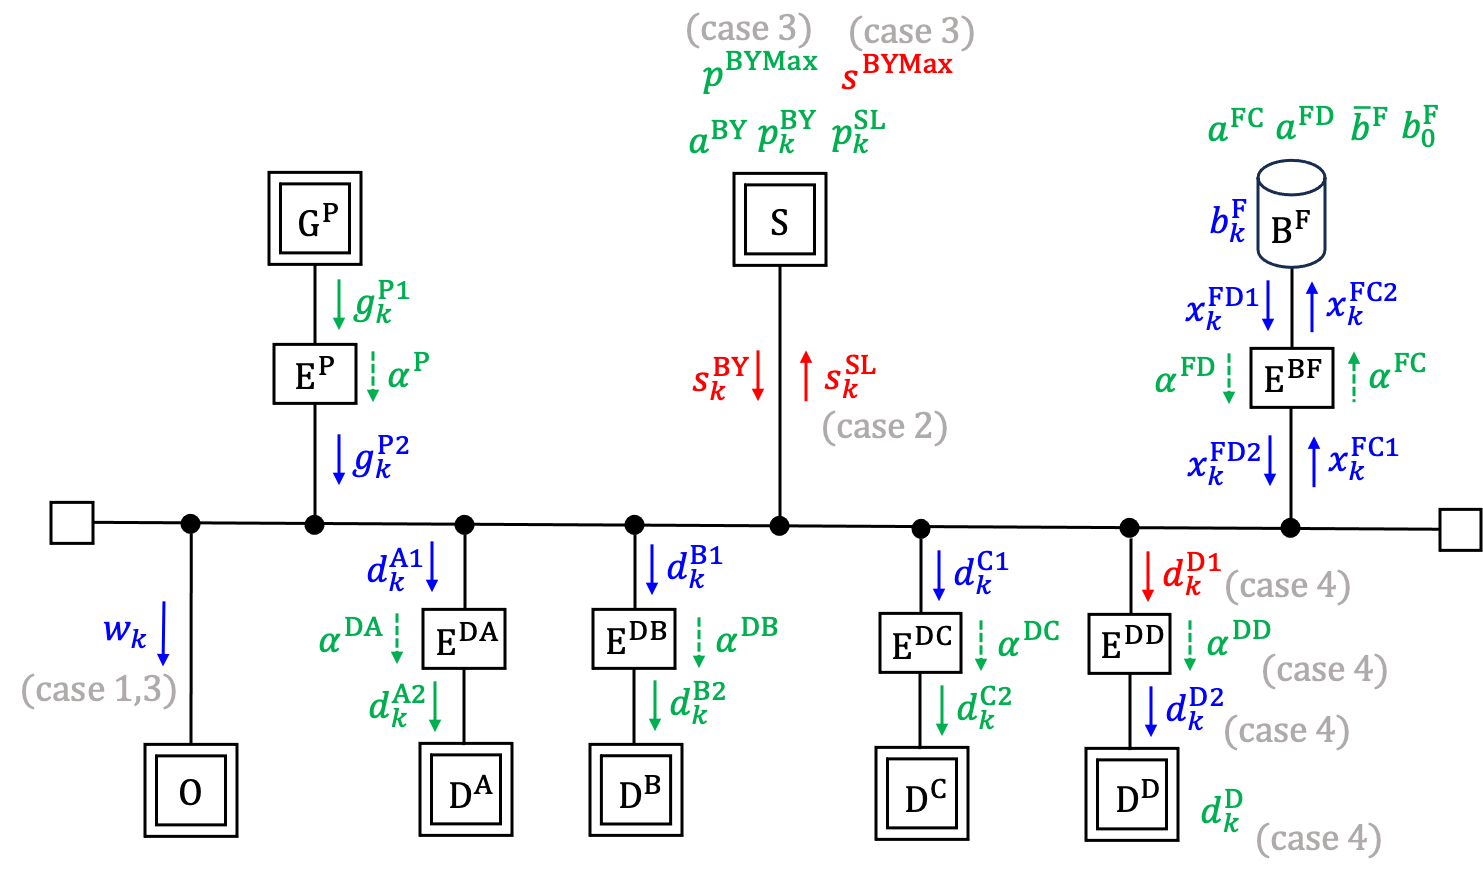
\includegraphics[width=140mm]{../figure/variables_lp.png}
 \caption{Configuration diagram of the target system(Linear Programming)}
 \label{fig:variables_lp}
\end{figure}

\section{目的関数}
最適化の目的は経済性の追求や環境価値の最大化など多岐にわたる．
ゆえに目的関数の定式化の方法は必ずしも一意に定まらない．
本研究では，対象となる工場の運用方針を考慮し以下の4つのケースを想定する．

買電コストを最小化するケース(以降「ケース1」とよぶ．)：
\begin{equation}
    \text{Minimize} \quad  \sum_{k=1}^{K}  ( p_k^{\rm{BY} } s_k^{\rm{BY}}  )．
 \label{eq:minimize_lp_1}
\end{equation}

余剰電力の売電を考慮し，金銭の正味の支出を最小化するケース(以降「ケース2」とよぶ．)：
\begin{equation}
    \text{Minimize} \quad  \sum_{k=1}^{K}  ( p_k^{\rm{BY} } s_k^{\rm{BY}} - p_k^{\rm{SL} } s_k^{\rm{SL}}  )．
 \label{eq:minimize_lp_2}
\end{equation}

基本料金を考慮し買電コストを最小化するケース（以降「ケース3」とよぶ．）：
 \begin{equation}
 	 \text{Minimize} \quad \sum_{k=1}^{K} ( p_k^{\rm{BY} } s_k^{\rm{BY}} + p^{\rm{BYMax} } s^{\rm{BYMax}} )．
 	 \label{eq:minimize_lp_3} 
\end{equation} 
なお，基本料金は契約電力に比例して決定される．実運用における契約電力は，当月を含む過去1年間の各月における最大需要電力
（30分間ごとの平均使用電力の最大値）のうち最も大きい値に基づいて決定されるが，
本研究では$K$期分における運用のみを評価対象とするため，
当該期間内における最大需要電力がそのまま契約電力を決定するものと仮定する．

支出を抑制しつつ，余剰電力の自己託送量をなるべく大きくするケース(以降「ケース4」とよぶ．)：
\begin{equation}
    \text{Minimize} \quad  \sum_{k=1}^{K}  ( p_k^{\rm{BY} } s_k^{\rm{BY}} - p^{\rm{D} } s_k^{\rm{D}}  )．
 \label{eq:minimize_lp_4}
\end{equation}


\section{制約条件}
\ref{sec:object_seiyaku}節で述べた事項を制約条件に書きかえたものを以下に列挙する．
ただし，特に断り書きがない場合，目的関数が(\ref{eq:minimize_lp_1})式〜(\ref{eq:minimize_lp_4})式のどのケースで表される場合について
も共通する制約条件である．また全ての変数は非負である．

\begin{itemize}
	\item 動線\\
		流入する電力と流出する電力の総和が等しいものとする(ケース1，ケース3の場合)
		\begin{equation}
			g^{\rm P2}_{k} + s^{\rm BY}_{k} 
 			- x^{\rm FC1}_{k} + x^{\rm FD2}_{k} 
 			- d^{\rm A1}_{k} - d^{\rm B1}_{k} - d^{\rm C1}_{k} - w_{k}= 0，
		 \quad
 		k=1,\dots,K
		~~
		\label{eq:line1}
		\end{equation}
		流入する電力と流出する電力の総和が等しいものとする(ケース2の場合)
		\begin{equation}
			g^{\rm P2}_{k} + s^{\rm BY}_{k} - s^{\rm SL}_{k}
 			- x^{\rm FC1}_{k} + x^{\rm FD2}_{k} 
 			- d^{\rm A1}_{k} - d^{\rm B1}_{k} - d^{\rm C1}_{k}  = 0，
		 \quad
 		k=1,\dots,K
		~~
		\label{eq:line23}
		\end{equation}
		流入する電力と流出する電力の総和が等しいものとする(ケース4の場合)
		\begin{equation}
			g^{\rm P2}_{k} + s^{\rm BY}_{k}
 			- x^{\rm FC1}_{k} + x^{\rm FD2}_{k} 
 			- d^{\rm A1}_{k} - d^{\rm B1}_{k} - d^{\rm C1}_{k}  = 0，
		 \quad
 		k=1,\dots,K
		~~
		\label{eq:line4}
		\end{equation}
	\item 蓄電池\\
		蓄電池の残量の推移についての関係式
		\begin{equation}
 			b_k^{\rm F} = \alpha^{\rm FT}b_{k-1}^{\rm F} + x_{k}^{\rm FC2} - x_{k}^{\rm FD1}
 			\quad
 			k=1,\ldots,K
			~~
			\label{eq:b_f}
		\end{equation}
		蓄電池の残量は常に定められた範囲内を外れないこと
		\begin{equation}
 			0 \le b^{\rm F}_{k} \le \overline{b}^{\rm F},
 			\quad
 			k=1,\ldots,K
			~~
			\label{eq:b_max}
		\end{equation}
		単位時間あたりの充放電電力は，最大出力を超過しないこと
		\begin{equation}
 			 x^{\rm FC2}_{k} \le a^{\rm FC},
 			\quad
 			k=1,\ldots,K
			~~
			\label{eq:x_fc}
		\end{equation}
		\begin{equation}
 			  x^{\rm FD1}_{k} \le a^{\rm FD},
 			\quad
 			k=1,\ldots,K
			~~
			\label{eq:x_fd}
		\end{equation}
	\item 商用電力系統\\
		任意の連続する30 分間の区間について，商用電力系統からの総買電力を一定量以下に制限すること
		(目的関数が\eqref{eq:minimize_lp_1},\eqref{eq:minimize_lp_2},\eqref{eq:minimize_lp_4}の場合)
		\begin{equation}
 			 \sum_{k'=30m}^{30m+29}s^{\rm BY}_{k'} \le  a^{\rm BY},
			 \quad
			 m=1,\ldots,\frac{K}{30}-1
			~~
			\label{eq:sMax}
		\end{equation}
		契約電力に関する関係式を満たすこと(ケース3の場合)
		\begin{equation}
 			\sum_{k'=30m}^{30m+29}s^{\rm BY}_{k'}   \le  s^{\rm BYMax},
 			\quad
 			m=1,\ldots,\frac{K}{30}-1
			~~
			\label{eq:sMax}
		\end{equation}
		
	\item 電力変換装置\\
		パワーコンディショナや変圧器などを介して電力を変換・送電する際，一定の変換効率に応じた電力損失が発生するものとする
		\begin{equation}
 			  g^{\rm P2}_{k} \le \alpha^{\rm P} g^{\rm P1}_{k} ,
 			\quad
 			k=1,\ldots,K
			~~
			\label{eq:gP1gP2}
		\end{equation}
		\begin{equation}
 			   d^{\rm A2}_{k} \le \alpha^{\rm DA} d^{\rm A1}_{k} ,
 			\quad
 			k=1,\ldots,K
			~~
			\label{eq:dA1A2}
		\end{equation}
		\begin{equation}
 			 d^{\rm B2}_{k} \le \alpha^{\rm DB} d^{\rm B1}_{k} ,
 			\quad
 			k=1,\ldots,K
			~~
			\label{eq:dB1B2}
		\end{equation}
		\begin{equation}
 			  d^{\rm C2}_{k} \le \alpha^{\rm DC} d^{\rm C1}_{k},
 			\quad
 			k=1,\ldots,K
			~~
			\label{eq:dC1C2}
		\end{equation}
		(ケース4式の場合)
		\begin{equation}
 			  d^{\rm D2}_{k} \le \alpha^{\rm DC} d^{\rm D1}_{k},
 			\quad
 			k=1,\ldots,K
			~~
			\label{eq:dD1D2}
		\end{equation}
	\item 自己託送先\\
		自己託送先の需要電力量を上回る送電を行わないこと(ケース4の場合)
		\begin{equation}
 			  d^{\rm D2}_{k} \le d^{\rm D}_{k},
 			\quad
 			k=1,\ldots,K
			~~
			\label{eq:dD1D2}
		\end{equation}
\end{itemize}

以上に示すように，電力グリッドの運用最適化問題は，目的関数および制約条件がすべて線形で記述された．よって本問題は
線形計画法によるアプローチで求解可能である．

